%%%%%%%%%%%%%%%%%%%% author.tex %%%%%%%%%%%%%%%%%%%%%%%%%%%%%%%%%%%
%
% sample root file for your "contribution" to a contributed volume
%
% Use this file as a template for your own input.
%
%%%%%%%%%%%%%%%% Springer %%%%%%%%%%%%%%%%%%%%%%%%%%%%%%%%%%


% RECOMMENDED %%%%%%%%%%%%%%%%%%%%%%%%%%%%%%%%%%%%%%%%%%%%%%%%%%%
\documentclass[graybox]{svmult}
\usepackage{etex}


%\usepackage[english]{babel}
%
\usepackage[utf8]{inputenc}
% choose options for [] as required from the list
% in the Reference Guide

\usepackage{mathptmx}       % selects Times Roman as basic font
\usepackage{helvet}         % selects Helvetica as sans-serif font
\usepackage{courier}        % selects Courier as typewriter font
\usepackage{type1cm}        % activate if the above 3 fonts are
                            % not available on your system
%
\usepackage{makeidx}         % allows index generation
\usepackage{graphicx}        % standard LaTeX graphics tool
\usepackage[size=small,labelfont=bf]{caption}
                             % when including figure files
\usepackage{multicol}        % used for the two-column index
\usepackage[bottom]{footmisc}% places footnotes at page bottom
\usepackage{pdflscape}
%\usepackage{rotating}
\usepackage{afterpage}
%\usepackage[disable]{todonotes}
\usepackage[colorinlistoftodos,prependcaption]{todonotes}
%\usepackage{todonotes}
\usepackage{subfigure}
\usepackage{setspace}
\usepackage{epstopdf}
\usepackage{flafter} %make sure that the floats are not placed 
%before their definition
\usepackage{times}
\usepackage{bm}
\usepackage{gensymb}  % for degree sign, e.g., temperature
\usepackage{amsmath}
\usepackage{amstext}
\usepackage{array}  %for define the fomats of columns in a table
\usepackage{dcolumn}
\usepackage[T1]{fontenc}
\usepackage{pgfplots}
\usepackage{multirow}
\usepackage{makecell}
\usepackage{tabularx}
\usepackage{adjustbox}
\usepackage{capt-of}
%\usepackage{marginnote}
\usepackage{xargs}   % Use more than one 
%optional parameter in a new commands
%\usepackage{siunitx} %for scientific 
%notation
%%we do this because of a bug of package floatrow
%\let\tmp\newinsert
%\let\newinsert\newbox
%\usepackage{floatrow}
%\let\newinsert\tmp
\usepackage{enumitem} %make items indent when using 
%\begin{enumerate}[(a)]
\usepackage{verbatimbox}  %for \addvbuffer
\usepackage{hyperref}
\usepackage{tikz}
\usepackage{xspace}
%\usepackage{pdfcomment}
%\newcommand*\circled[1]{\tikz[baseline=(char.base)]{
%		\node[shape=circle,draw,inner sep=1pt] (char) {#1};}}
%\newcommand*\circledtwo[1]{\tikz[baseline=(char.base)]{
%		\node[shape=circle,draw,inner sep=0.1pt] (char) {#1};}}
% \newcommand{\ml}{\ensuremath{M_+}\xspace}
% \newcommand{\ms}{\ensuremath{M_-}\xspace}



\usepackage[backend=bibtex,
bibstyle=authoryear, %without indices before names; year after 
%names
%style=authoryear,
citestyle=authoryear,
maxbibnames=20,maxcitenames=2,
firstinits=true,
%terseinits=true, %remove periods after initials of first names
%style=apa, %
%sorting=ydnt, %Sort bibliography by year (descending), name, 
%title
doi=false,isbn=false,url=false,
eprint=false,dashed=false]{biblatex}

%\renewcommand*{\bibfont}{\small} %set the font size of the 
%references
%\renewcommand*{\nameyeardelim}{\addspace} %\remove the comma 
%between author and year citations
%\renewcommand*{\revsdnamepunct}{} %remove commas between last 
%%and first names in bibliography
%\renewcommand{\labelnamepunct}{\addspace} %remove the 
%%punctuation after the year in bibliography
%\renewcommand{\finentrypunct}{} %remove the full stop at the 
%%end of each bibliography entry
\renewcommand*{\revsdnamepunct}{} %remove commas between last 
%and first names in bibliography

%remove "In:" for articles in bibliography
\renewbibmacro{in:}{\ifentrytype{article}{}
	{\printtext{\bibstring{in}\intitlepunct}}} 

\addbibresource{References.bib}



\newcommand{\mypar}[1]{\bigskip\noindent\textbf{#1.}~}

\newcommand{\e}[1]{\times 10^{#1}}

\graphicspath{{figures/}}
\DeclareMathAlphabet{\mathpzc}{OT1}{pzc}{m}{it}

%For the references, the following commands make the titles 
%lowercase while keep the initial letters of journal names 
%uppercase
\DeclareFieldFormat{titlecase}{\MakeSentenceCase*{#1}}
\newbibmacro*{journal}{%
	\iffieldundef{journaltitle}
	{}
	{\printtext[journaltitle]{%
			\printfield[myplain]{journaltitle}%
			\setunit{\subtitlepunct}%
			\printfield[myplain]{journalsubtitle}}}}
\DeclareFieldFormat{myplain}{#1}

%Remove the quotation marks for the titles in the reference
\DeclareFieldFormat[article,inbook,incollection,inproceedings,patent,thesis,unpublished]{citetitle}{#1}
\DeclareFieldFormat[article,inbook,incollection,inproceedings,patent,thesis,unpublished]{title}{#1}
\DeclareNameAlias{author}{last-first}

%%Using \DeclarePairedDelimiter from mathtools, you could define 
%%macros \ceil and \floor, which will scale the delimiters 
%%properly (if starred):
%\usepackage{mathtools}
%\DeclarePairedDelimiter\ceil{\lceil}{\rceil}
%\DeclarePairedDelimiter\floor{\lfloor}{\rfloor}

\pgfplotsset{
	compat=newest,
	xlabel near ticks,
	ylabel near ticks
}


\newcommandx{\marginalcomment}[2][1=]{\todo[linecolor=blue,backgroundcolor=blue!25,bordercolor=blue,#1]{#2}}

\renewcommand{\textfraction}{0.01}
\renewcommand{\topfraction}{0.99}
\renewcommand{\bottomfraction}{0.99}
\renewcommand{\dbltopfraction}{0.99} % fit big float above 
%2-col. text
%\renewcommand\thesection{\arabic{section}}
%\renewcommand\thesubsection{\thesection.\arabic{subsection}}



% see the list of further useful packages
% in the Reference Guide

\makeindex             % used for the subject index
                       % please use the style svind.ist with
                       % your makeindex program

%%%%%%%%%%%%%%%%%%%%%%%%%%%%%%%%%%%%%%%%%%%%%%%%%%%%%%%%%%%%%%%%%%%%%%%%%%%%%%%%%%%%%%%%%

\begin{document}

\title*{Continuous Generalization of Buildings}
\titlerunning{Continuous Generalization of Buildings}
% Use \titlerunning{Short Title} for an abbreviated version of
% your contribution title if the original one is too long
\author{Dongliang Peng and Guillaume Touya}
% Use \authorrunning{Short Title} for an abbreviated version of
% your contribution title if the original one is too long
\institute{
	Dongliang Peng 
	\at Chair of Computer Science I, University of W\"urzburg, 
	Germany \\
	\email{dongliang.peng@uni-wuerzburg.de}
	\and
	% 
	Guillaume Touya
	\at COGIT, IGN, France \\
	\email{guillaume.touya@ign.fr}
}
%
% Use the package "url.sty" to avoid
% problems with special characters
% used in your e-mail or web address
%
\maketitle

\newcommand{\myabstract}{We propose a method to continuously 
	generalize buildings from a given start scale to a smaller goal scale. 
	%
	If several buildings are close to each other at the start 
	scale, we bridge them by line segments and merge the several buildings into 
	one 
	building.
	For each building, either an original one or a merged one, at the start 
	scale, 
	we generate its target shape at 
	the goal scale by enlarging and simplifying. 
	Then we grow the building to the target shape.
	%
	After finishing the growing, we can take the goal scale as the 
	start scale and repeat the process.
	\newline\indent
	The advantages of our method are as follows. First, the buildings 
	are enlarged continuously. At the same time, they are simplified. 
	Second, we ensure that the distance between any pair of two buildings is 
	always larger than a specified threshold.}





\abstract*{\myabstract}

\abstract{\myabstract}


\keywords{Text, Text}

\section{Introduction}
\label{sec:Introduction}


Digital maps such as Google Maps and OpenStreetMap support zooming by 
displaying maps at different levels. 
This discrete strategy may results in sudden changes, which annoy users.
To provide better zooming experience, continuous generalization aims to 
produce 
a sequence of maps with small incremental changes.
To realize continuous generalization, \textcite{Sester2005_CG} discussed some 
generalization operators for buildings and proposed to morph a building 
between 
its forms at different levels. Morphing has been used to generate intermediate 
representations for two representations at different scales 
\parencite{mnwb-mpstc-08,Peng2013_LSA,Deng2015,Peng2016_Admin}. 
Also aiming at 
realize continuous generalization, \textcite{Chimani2014_Eat} generated a good 
selection sequence for road networks, and 
\textcite{Peng2017_AStar} tried to compute optimal aggregation sequences for 
land-cover areas.

When users zoom out on digital maps, buildings become closer with each other 
and buildings themselves become smaller. 
In order to make sure that the map is 
easily perceived \parencite{Weibel1997}, small building should be eliminated, 
some building should be enlarged, and buildings close to each other should be 
aggregated.
Although algorithms of simplifying buildings have been studied, e.g., 
\textcite{Buchin2011_Simp,haunertwolff2010}, problems become more complicated 
when we have to aggregate buildings simultaneously.
In order to aggregate, we should first group the buildings.

$\bar{a}$




\bigskip

The papers we may review:   
\textcite{vanSmaalen2003, Buchin2016, Chaudhry2008, Stoter2009},

Rules for building simplification; see \textcite{Lee2005}

Straight skeletons for map generalization: 
\textcite{Gold2003,Matuk2006}

Geometric Simplification of Administrative Borders With Mixture 
of
Irregular and Orthogonal Segments \parencite{Samsonov2016}

\citetitle{Damen2008} \parencite{Damen2008}

An example of enlargement in aggregation: \citetitle{Neun2005}

Using MST to group buildings: \textcite{Zhang2013, 
Cetinkaya2015,Deng2017,Regnauld1996}



\section{Method}

We grow all the buildings with the same speed.


If several buildings are close to each other at the start 
scale, we bridge them by line segments and take the merge of these 
buildings 
and bridges as one building.
For each building, either an original one or a merged one, at the start 
scale, 
we generate its target shape at 
the goal scale by enlarging and simplifying. Then we grow the  
building to the target shape. 

\subsection{Growing}
If several buildings are close to each other at the start 
scale, we bridge them by line segments and take the merge of these 
buildings 
and bridges as one building.
For each building, either an original one or a merged one, at the start 
scale, 
we generate its target shape at 
the goal scale by enlarging and simplifying. Then we grow the  
building to the target shape. 
%
After finishing the growing, we take the goal scale as the 
start scale and repeat our continuous generalization.
\newline\indent
Our contribution is as follows. First, the buildings 
are enlarged continuously. At the same time, they are simplified. 
Second, we ensure that the distance between any pair of two buildings is 
always larger than a specified threshold.

If we grow a building with radius $d_\mathrm{G}$, some part of a building will 
grow at most $2d_\mathrm{G}$.
The length of a bridge can be as large as
\begin{equation}
\label{eq:BridgeLength}
l_b=4d_\mathrm{G}+d_\epsilon.
\end{equation}
%\todo[inline]{$d_\mathrm{G}$ or $D_\mathrm{G}$?}

\subsection{Simplification}
we use a buffer-based method, similar to \textcite{Damen2008,Meijers2016}, to 
simplify our grown buildings.

We tried simplifying using Douglas--Peucker algorithm \parencite{Douglas1973}, 
but we hoped to remove more points. We found that Imai--Iri 
algorithm \parencite{ImaiIri1988} fit our needs well.

Imai--Iri algorithm finds all the valid shortcuts, and then 


\subsection{Parameters for growing and simplifying}
The start scale is $1:S_\mathrm{s}$, and the goal scale is $1:S_\mathrm{g}$ 
($S_\mathrm{g}>S_\mathrm{s}$).
The area of a building should be larger than $a$ mm$^2$ on map.
A square at the start scale has area $a S_\mathrm{s}^2$ mm$^2$ at least.
A square at the goal scale has area $a S_\mathrm{g}^2$ mm$^2$ at least.
The difference of the side lengths is $\sqrt{a} (S_\mathrm{g}-S_\mathrm{s})$ 
mm.
Therefore, a square on the start map needs to grow $\frac{1}{2}\sqrt{a} 
(S_\mathrm{g}-S_\mathrm{s})$ mm in order to survive.
In order to eliminate some small buildings, we define our growing distance as
\begin{equation}
\label{eq:d_G}
	d_\mathrm{G}=\frac{\lambda}{2}\sqrt{a} (S_\mathrm{g}-S_\mathrm{s}) \text{ 
	mm} \quad 0 < \lambda <1,
\end{equation}
where variable $\lambda$ is our growing factor. A larger $\lambda$ results in  
fewer buildings to be eliminated, and vice versa.

\begin{figure}[tb]
	\centering
	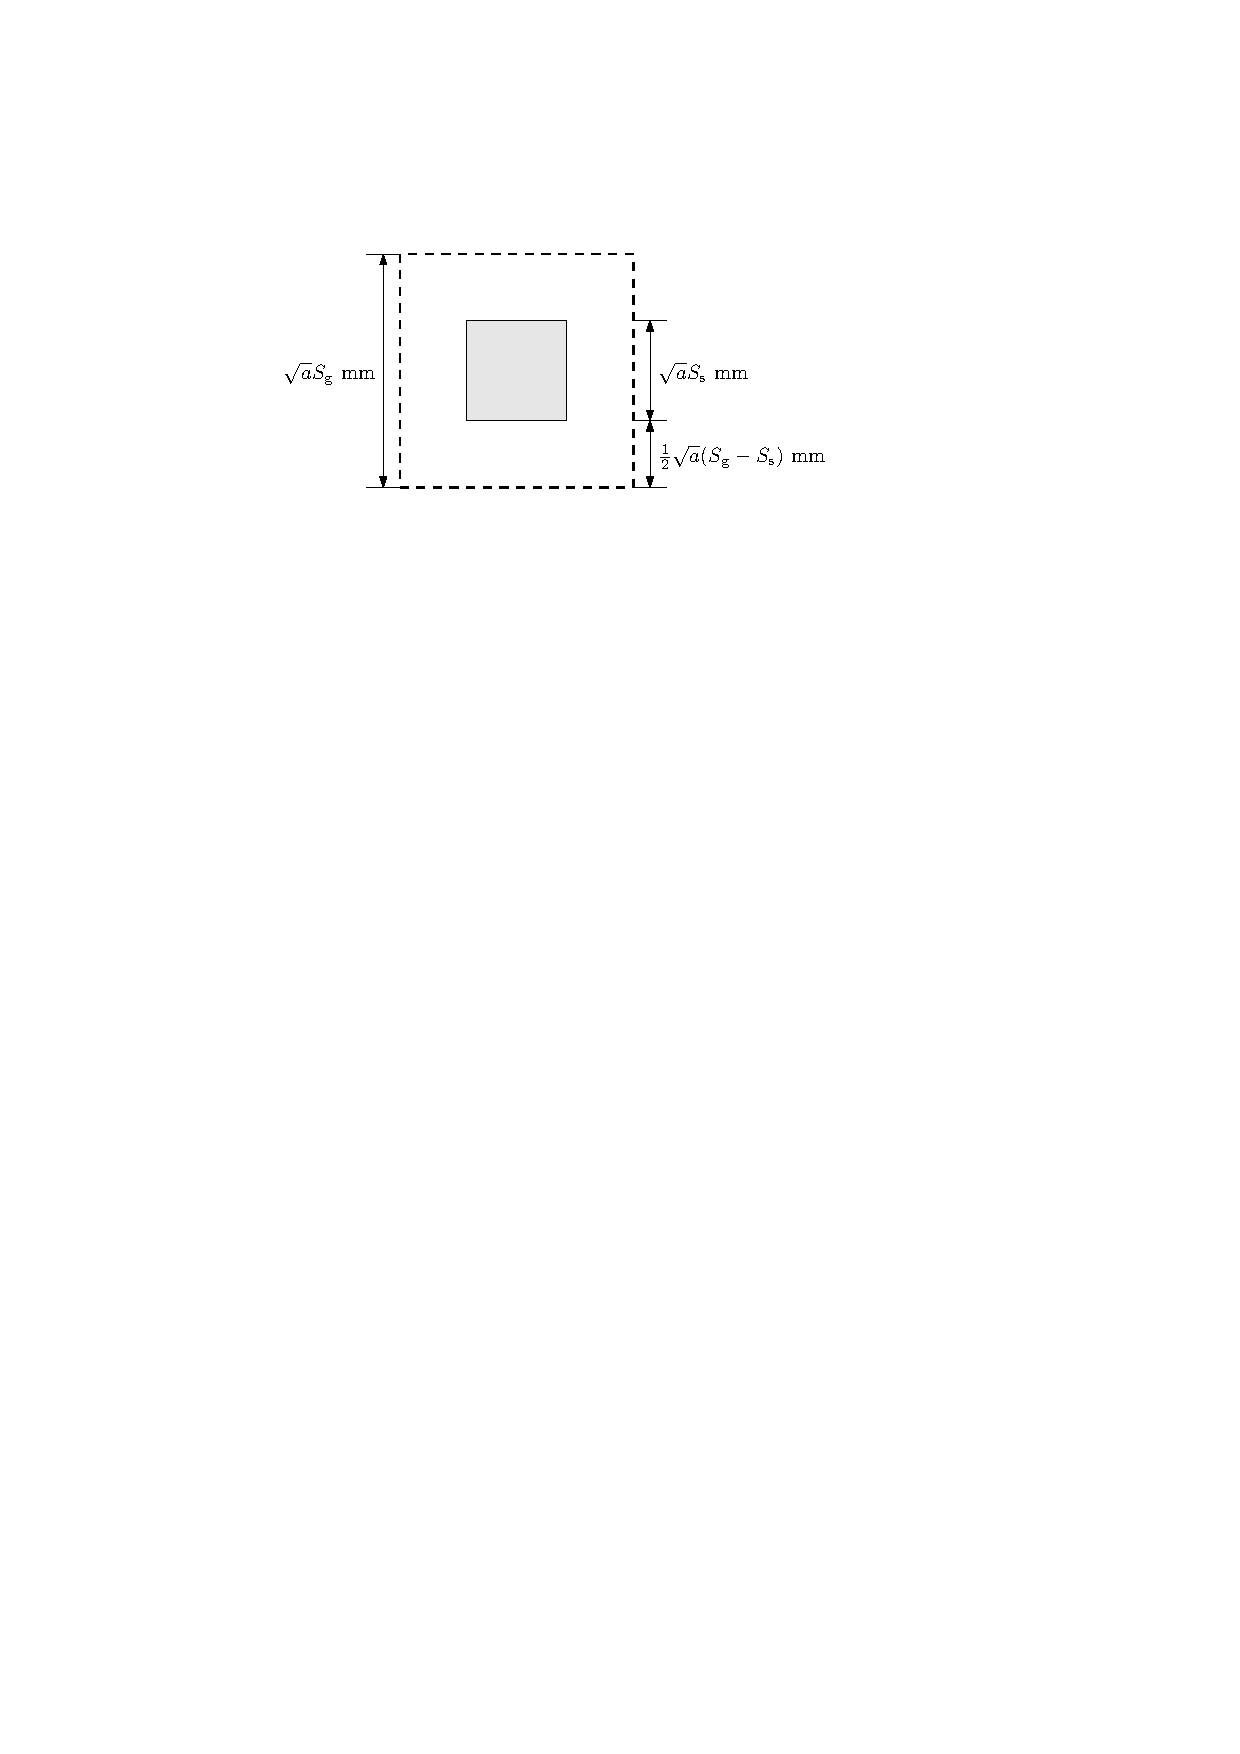
\includegraphics{Growth}
	\caption{Growth.}
	\label{fig:Growth}
\end{figure}

The distance between two buildings should be larger than a threshold, say, 
$\epsilon$ mm on map \parencite{Stoter2009}.
In order to make the shape of a building simpler, we simplify buildings 
using the Douglas--Peucker algorithm \parencite{Douglas1973} with preservation 
of right angles.
To avoid using too many thresholds, we also use $\epsilon$ mm for the 
simplification algorithm, hence the real threshold distance 
is
\begin{equation}
\label{eq:d_epsilon}
d_\epsilon= \epsilon  S_\mathrm{g}.
\end{equation}

If we insist on that we should observe 
the growing, say, $x \% (0<x<100)$ of the time at least, then we should make 
sure that
\begin{equation}
\label{eq:a_limit}
\frac{d_\mathrm{G}}{d_\mathrm{G}+d_\epsilon} \ge x \%.
\end{equation}
Using $d_\mathrm{G}$ and $d_\epsilon$ from Eqs.~\ref{eq:d_G} 
and~\ref{eq:d_epsilon}, we transform Eq.~\ref{eq:a_limit} to
\begin{equation}
a \ge \Big(\frac{2 \epsilon S_g x}{\lambda (100-x) (S_g-S_s)}\Big)^2
\end{equation}
\textcite{Stoter2009} used $0.2$ mm as minimal distance between two buildings 
on a map. We set our $\epsilon=0.2$.
We also require 
that $S_g \ge 2 S_s$, which means $S_s \le \frac{1}{2} S_g$.
On one hand, we should have a large $x$ so that we will see the 
growing most of the time.
On the other hand, we wish to keep bridges short as bridges are intrusions to 
our map, which means we should have a small $x$ and a large $\lambda$ so that 
we will have a small 
$a$ (according to Eq.~\ref{eq:a_limit}), a small $d_\mathrm{G}$ (according to 
Eq.~\ref{eq:d_G}), and finally a small $l_b$ (according to 
Eq.~\ref{eq:BridgeLength}). Also we should have a small $x$ and a large 
$\lambda$ as our $a$ is already much larger than $0.16$ mm$^2$ on 
map, which is the area limit used by \textcite{Stoter2009}. As a result, we 
set 
$\lambda=0.8$ and $x=\frac{2}{3} \cdot 100$.
Using these setting, we have
\begin{equation}
a \ge 4.
\end{equation}
according to Eq.~\ref{eq:a_limit}.




Therefore, we may grow up to distance 
\[
D_\mathrm{G} = d_\mathrm{G} + d_\epsilon.
\]
Fig.~\ref{fig:ExtraGrowth} shows such an enlargement and simplification, 
where  
variable $d_\mathrm{e} (\le d_\epsilon)$ is the extra growing distance.


\textcite{Chaudhry2008} thought that a hole of a settlement should be at least 
$0.5$ km$^2$ for a map at scale $1:250{,}000$, which means that the hole is at 
least $8$ mm$^2$ on map. Following their setting, we shrink a hole and 
eliminate the hole once its size is smaller than $8$ mm$^2$ on map.







%
%A hole has area less than $\pi D_\mathrm{G}^2$ can be filled by growing. 
%A hole has area 
%slightly more than $\pi D_\mathrm{G}^2$ will become a very small hole after 
%growing with 
%distance $D_\mathrm{G}$. In order to avoid small holes, we do not fill a hole 
%unless the 
%area of the hole on the start map is smaller than $\pi D_\mathrm{G}^2$. Note 
%that we do 
%not fill a hole even if the hole has a large area because a large hole may be 
%split into several small holes by filling. 
%Although our intermediate results may violate the rule that a hole should be 
%at 
%least some size, we try to avoid the violation for a map at a goal scale.
%\textcite{Chaudhry2008} thought that a hole of a settlement should be at 
%least 
%$0.5$ km$^2$ for a map at scale $1:250{,}000$, which means that the hole is 
%at 
%least $8$ mm$^2$ on the map. Following their setting, we wish to have $\pi 
%D_\mathrm{G}^2 \ge 8 S_g^2$.
%
%
%Now we discuss how to set the parameters according to our requirements. 
%First, 
%we wish to increase $d_\mathrm{G}/d_\epsilon$. Most part of a building will 
%grow $d_\mathrm{G}$. Only a small part will continue growing after the 
%building 
%has grown $d_\mathrm{G}$. To ensure that we can see the growing most of the 
%time, we want to have a large $d_\mathrm{G}/d_\epsilon$.
%
%
%
%
%
%We cannot fulfill all the requirements. 

\begin{figure}[tb]
	\centering
	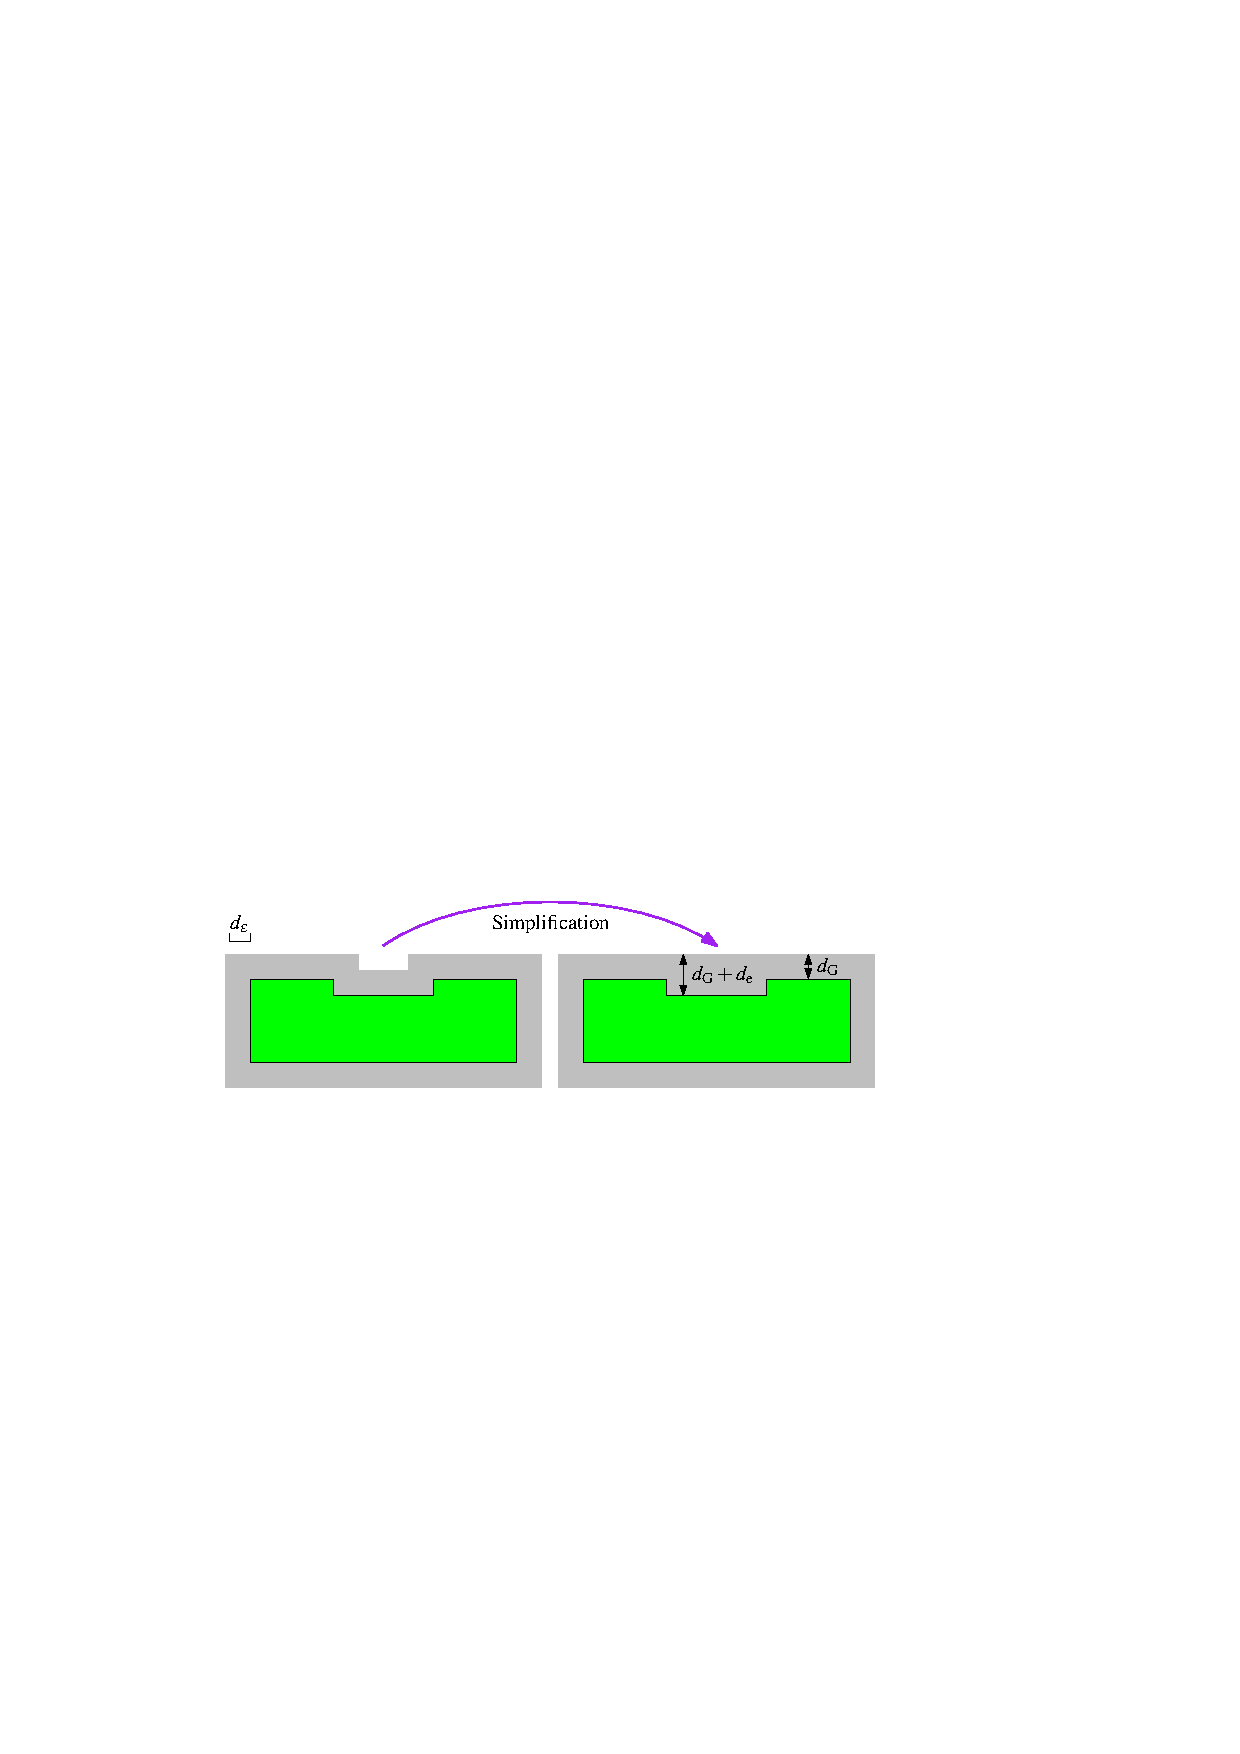
\includegraphics{ExtraGrowth}
	\caption{In the left figure, the green polygon represents a building, and 
	the gray polygon is the enlargement of the building. In the right 
	figure, the gray polygon has been simplified to a rectangle. In order to 
	fill the rectangle, most parts of the (green) building needs to grow with
	distance $d_\mathrm{G}$, but the pit needs to grow with $d_G + 
	d_\mathrm{e}$, 
	where $d_\mathrm{e}$ is the extra growing distance.}
	\label{fig:ExtraGrowth}
\end{figure}


\begin{figure}[tb]
	\centering
	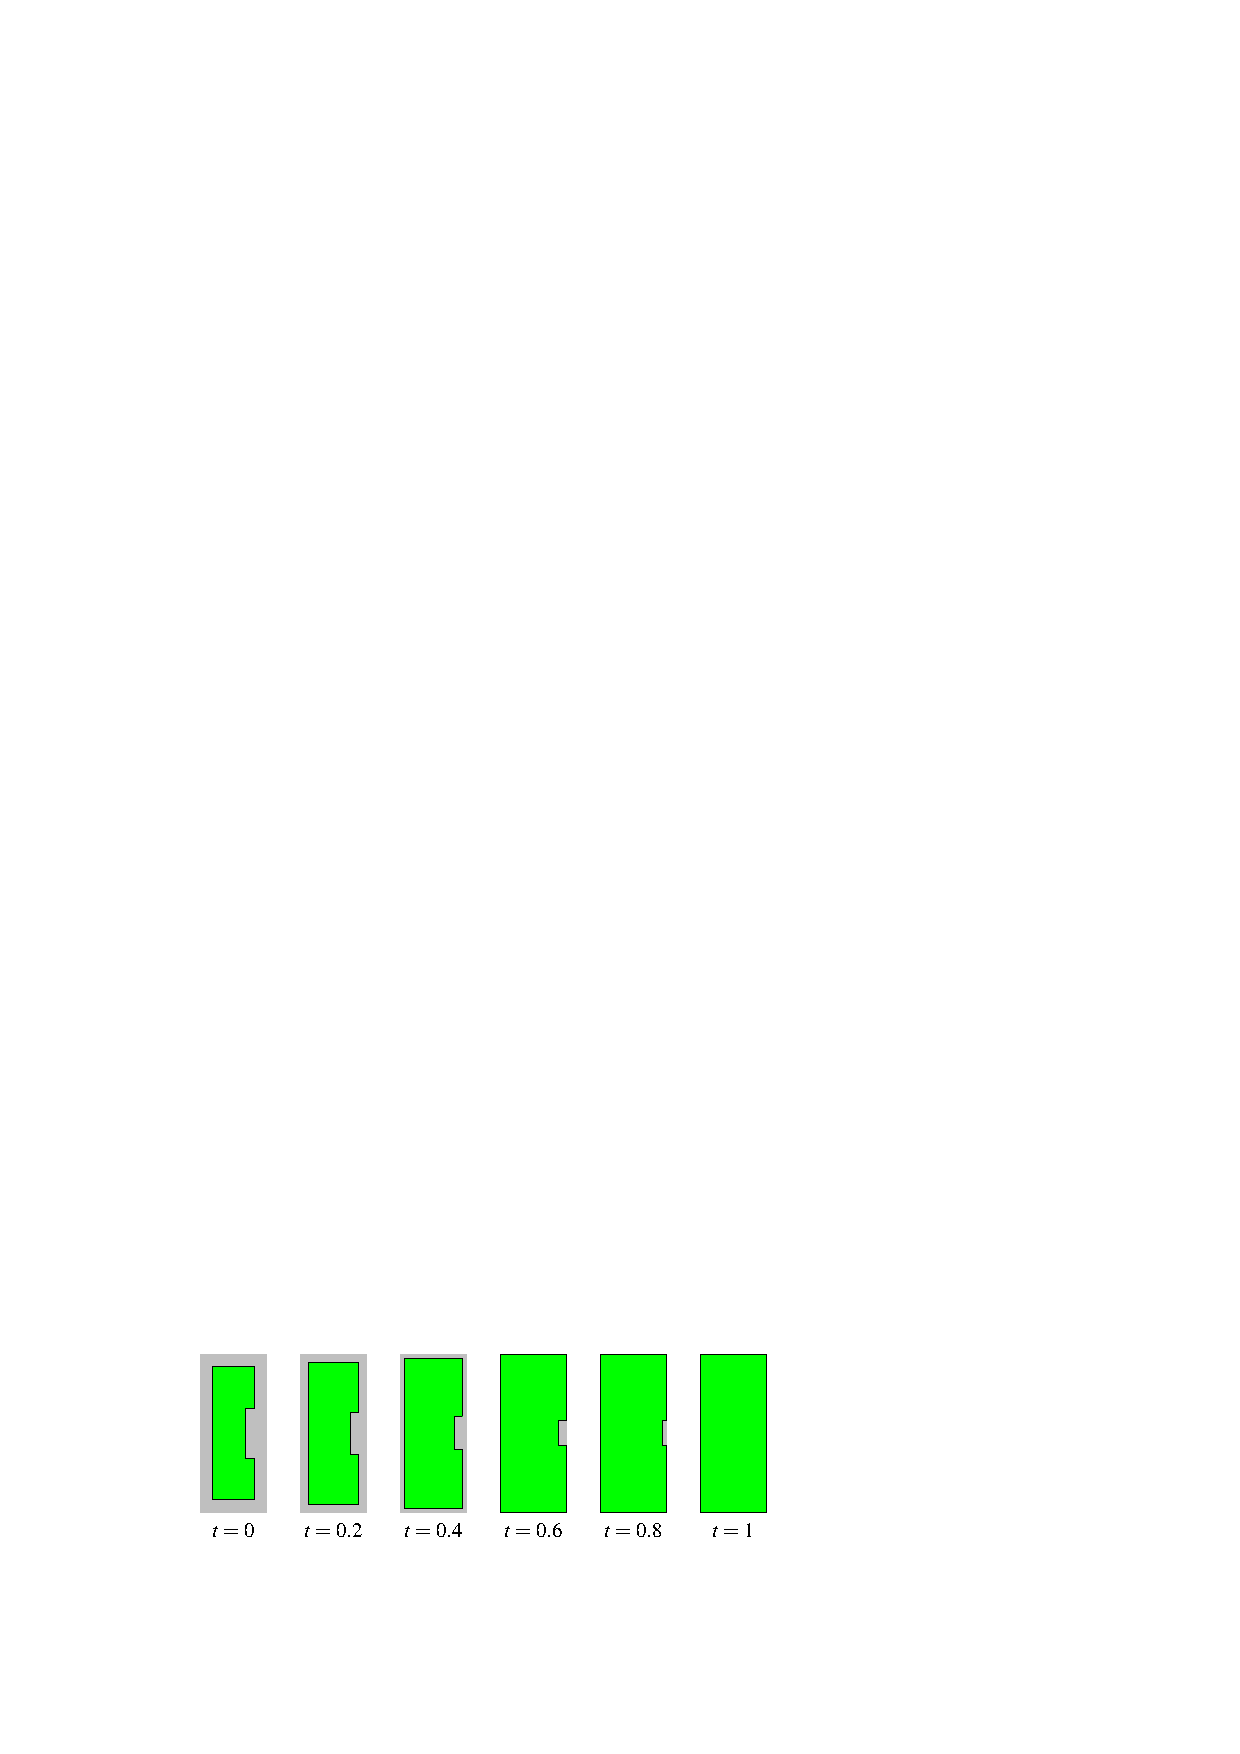
\includegraphics{GrowingExample}
	\caption{GrowingExample.}
	\label{fig:GrowingExample}
\end{figure}

\section{Section Title}
\label{sec:AStarAlgorithm}

\mypar{Notation}
Text. 

\subsection{Text}
\label{sec:Formalizing}



\section{Conclusions}
\label{sec:Conclusions}

Because of our aggregation with skeletons and original 
buildings, we may have too many details in the intermediate 
results.

Some buildings are too small to be eroded. We have to generate 
squares or MBR?

To make it more efficient for on line displaying, we may need 
some external memories. First, we store the data at some key 
scales so that we may start a generalization from the immediate 
larger scale; $O(n)$ space. Second, we store the target shape 
for each building; $O(n)$ space. Third, we store the aggregation 
time and the target form for the aggregated shape; $O(n^2)$ 
space if we count vertex number.
%
The displaying time is dependent on buffering and clipping. The 
two operators are from library Clipper. The efficiency of the 
buffering function of this library has been evaluated by 
\textcite{Palfrader2015}.

One can also discuss about our growing speed.

We our intermediate results may violate more cartographic rules, but we try to 
make the results at goal scales violate as few rules as possible.

Ideally, for a rectangle, the ratio of width to height should be kept.

The closest place of two buildings before enlarging is not necessarily the same 
as the closest place after enlarging. 

\todo[inline]{consider multi bridges; consider transparency of bridges in 
stead 
of enlarging}

\printbibliography
%\bibliographystyle{plainnat}
%%	\bibliography{References}
%\input{referenc}
\end{document}